\documentclass{beamer}
\usetheme{UASLP1}
\usepackage[utf8]{inputenc}
\usepackage[T1]{fontenc}

%% Use any fonts you like.
\usepackage{helvet}

\title{WRAP UP}
\subtitle{SFB R-Workshop}
\author{Alina Koppold \\ Rachel Sjouwerman}
\date{\tiny{\today}}
\institute{\url{a.koppold@uke.de}\\ \url{r.sjouwerman@uke.de}}

\begin{document}
\begin{frame}[plain,t]
\titlepage
\end{frame}

\begin{frame}{Your Data}
    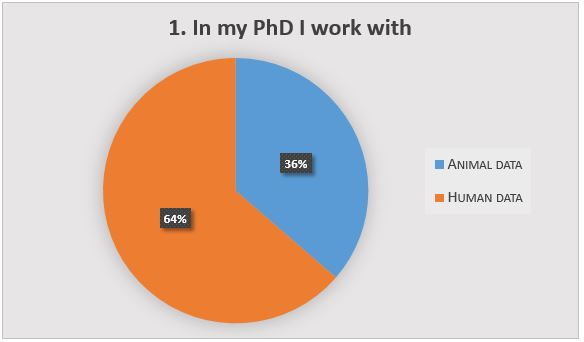
\includegraphics[width = 9.5cm]{um1.JPG}
\end{frame}

\begin{frame}{Your Data}
    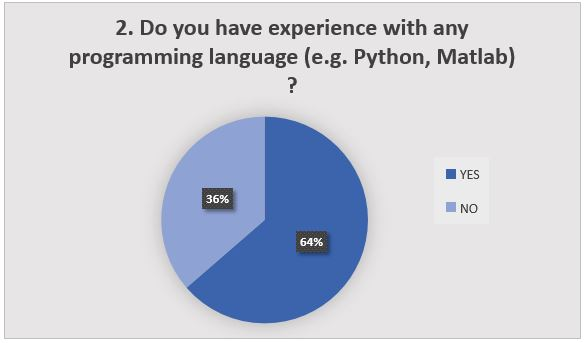
\includegraphics[width = 9.5cm]{um2.JPG}
\end{frame}

\begin{frame}{Your Data}
    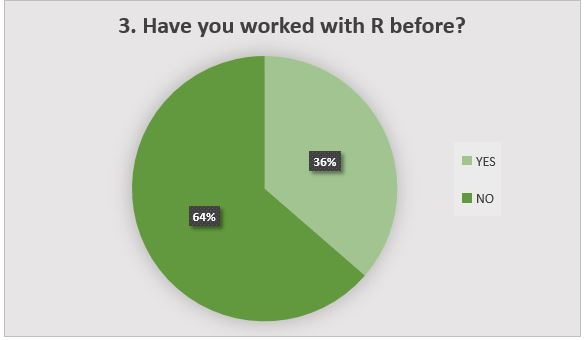
\includegraphics[width = 9.5cm]{um3.JPG}
\end{frame}

\begin{frame}{Your Data}
    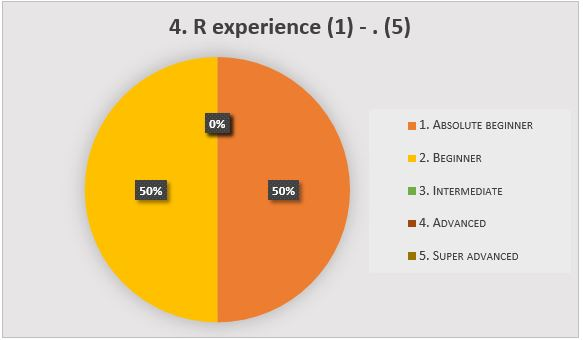
\includegraphics[width = 9.5cm]{um4.JPG}
\end{frame}


\begin{frame}{RAQ}
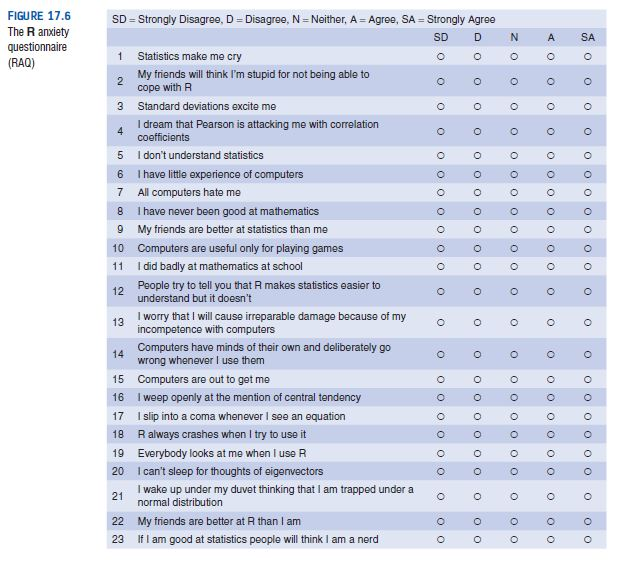
\includegraphics[width = 9cm]{RAQ_R_anxiety_quest.JPG}
\end{frame}

\begin{frame}{Logical Operators}
    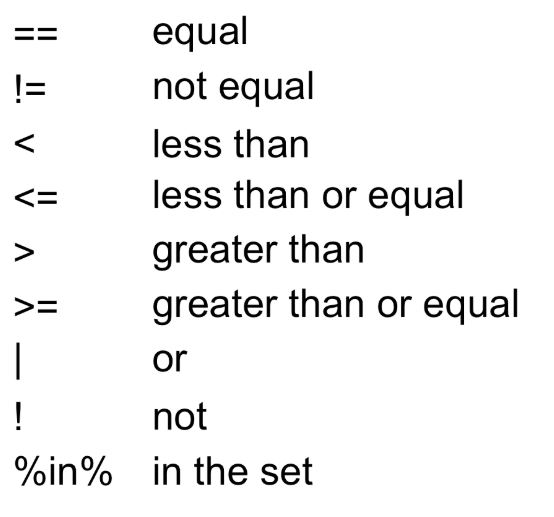
\includegraphics[width = 7cm]{lo.JPG}
\end{frame}

\begin{frame}{Logical Operators}
    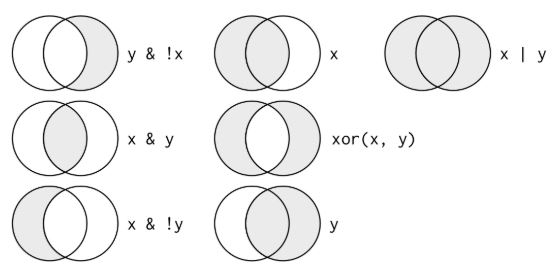
\includegraphics[width = 9.5cm]{lo2.JPG}
\end{frame}

\begin{frame}{Wide vs. Longformat}
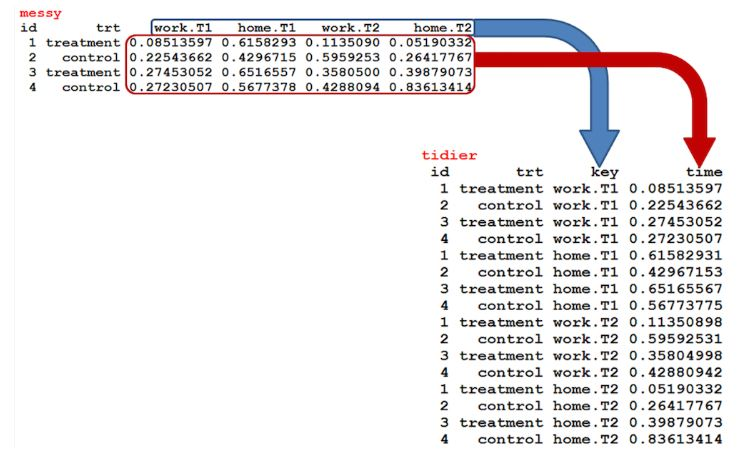
\includegraphics[width = 10cm]{gather.JPG}
\end{frame}



\section{Summary}
\begin{frame}
\frametitle{Summary}
\framesubtitle{Topics of today}
\frametitle{Overview}

\begin{columns} 
      \column[t]{.50\textwidth} 
    \begin{itemize}
    \item \textsc{Data visualization}
    \item \textsc{Data transformation }
    \item \textsc{Data preprocessing}
    \item \textsc{Plotting }
    \item \textsc{Statistics}
    \end{itemize} 
     \column[t]{.50\textwidth} 
     \begin{figure}
    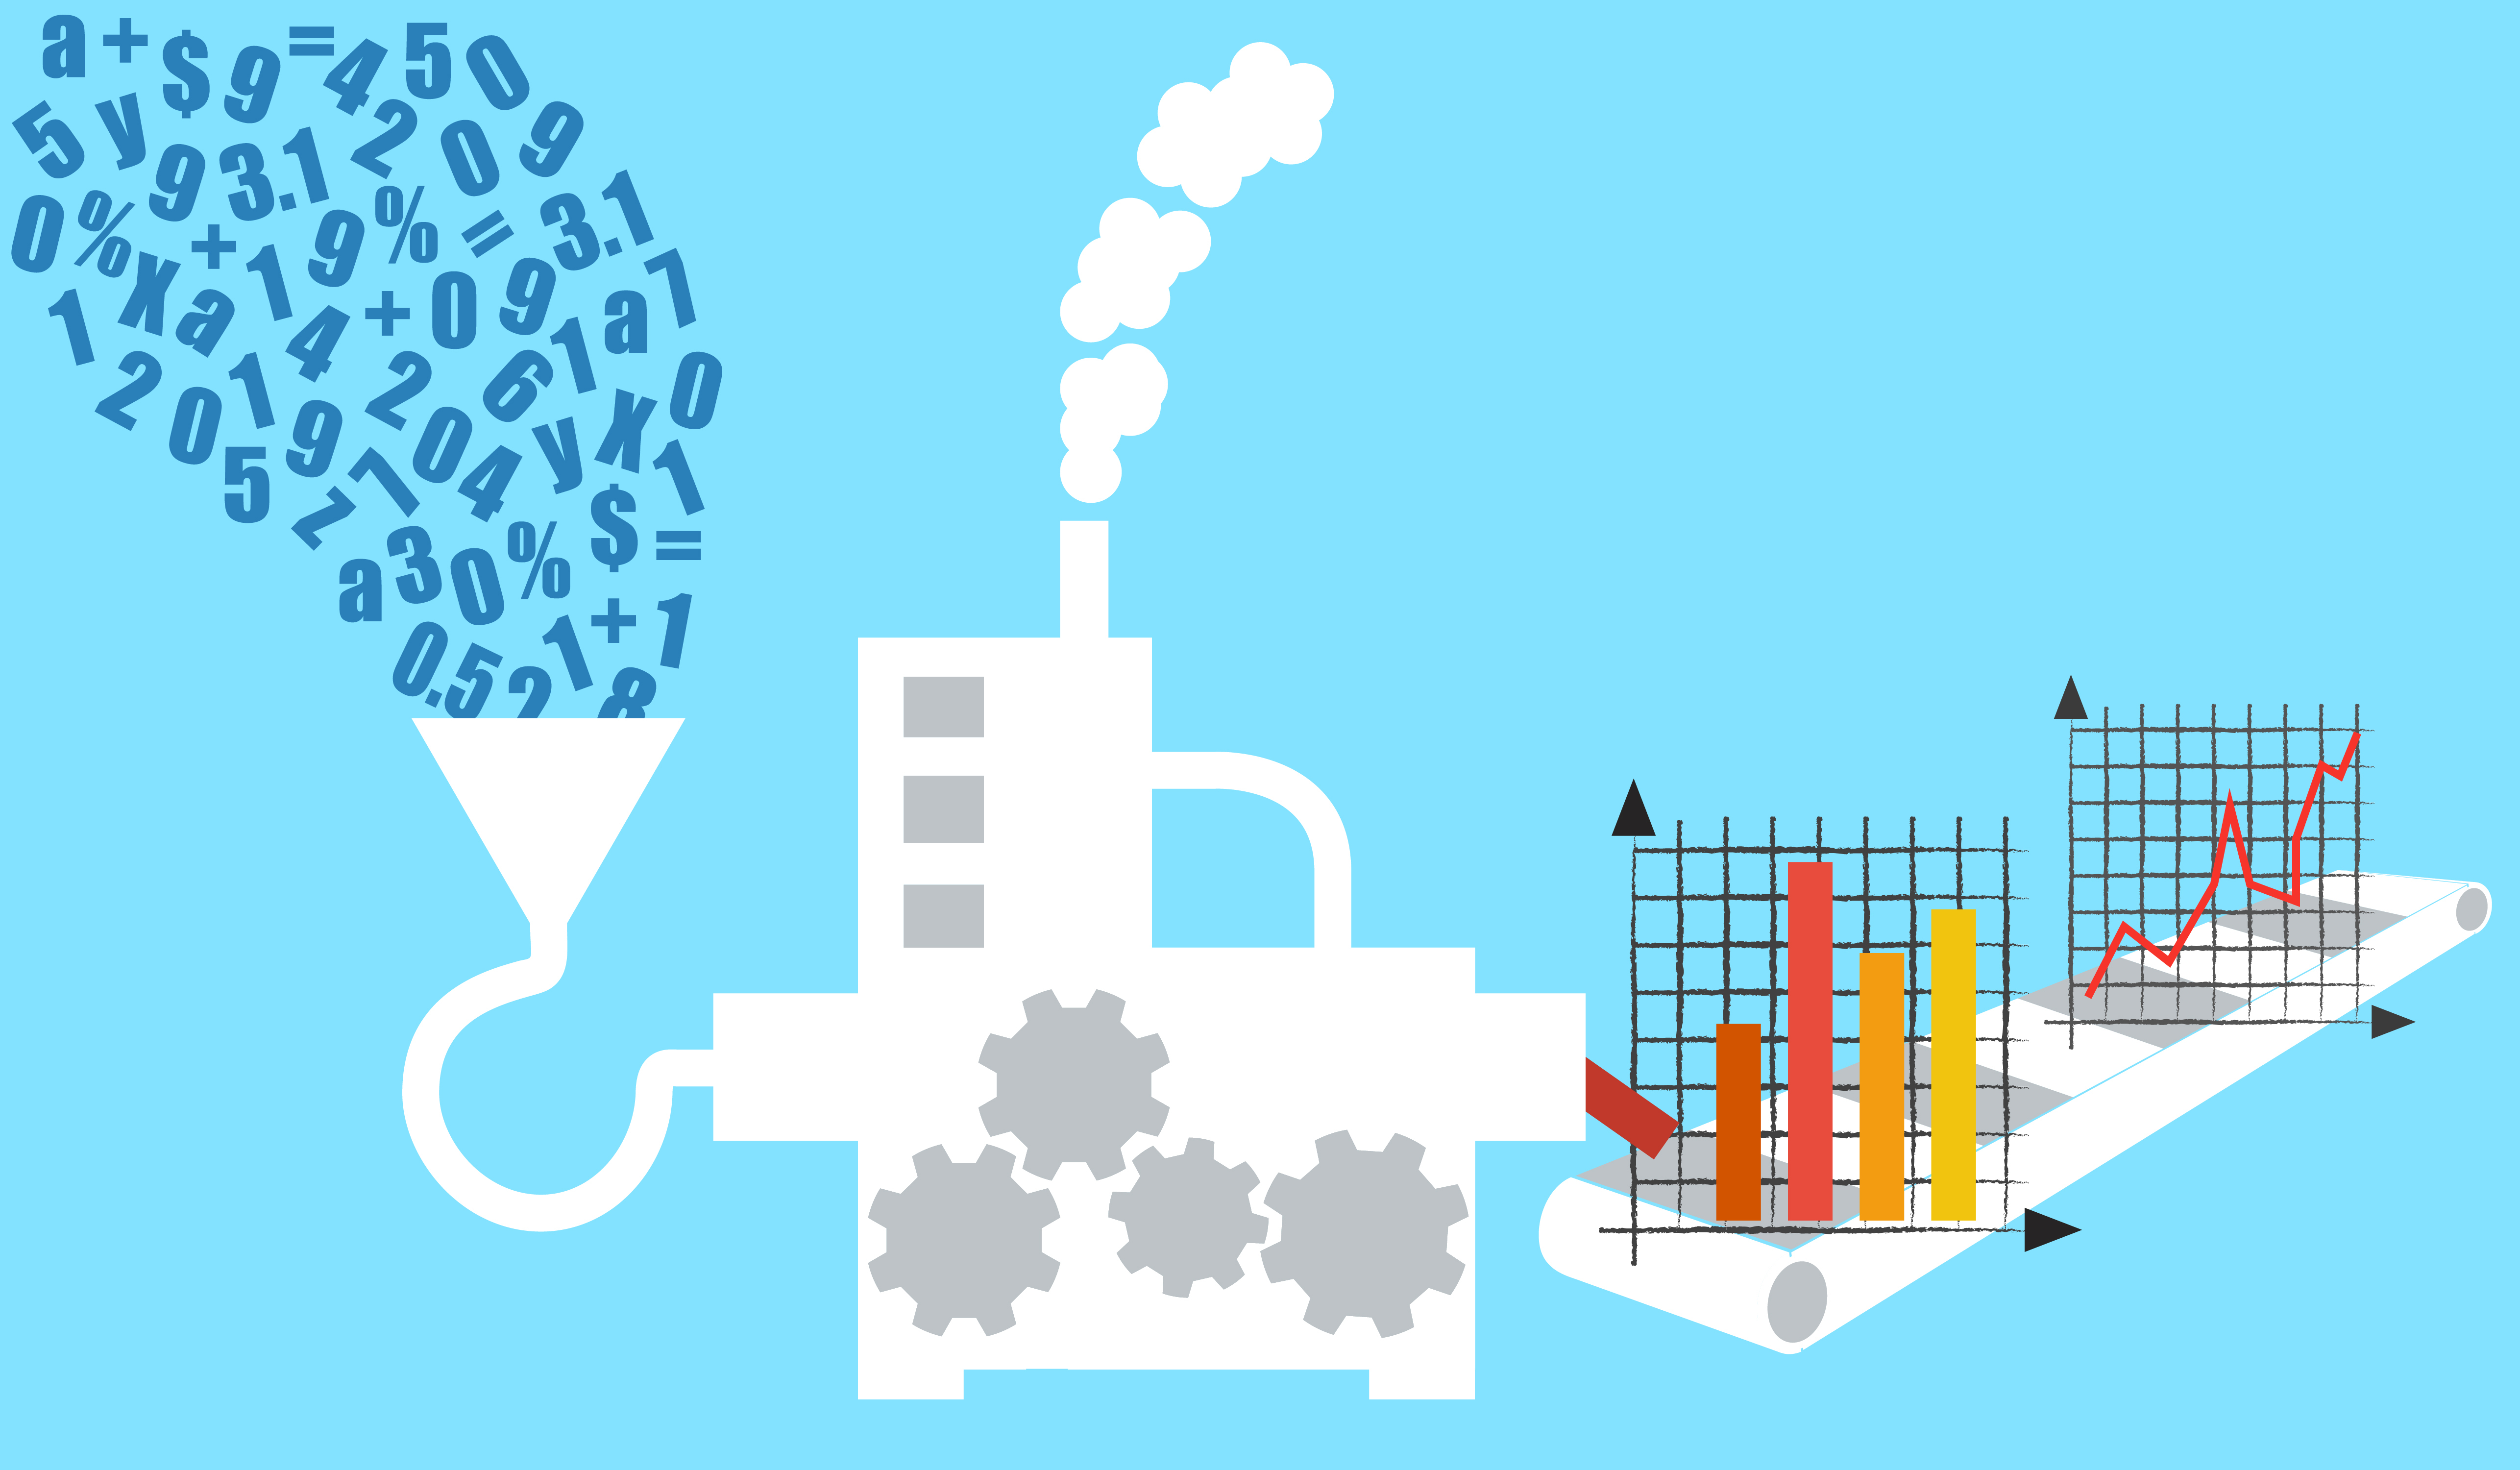
\includegraphics[width =4cm]{data_processing.jpg}
    \vspace{3cm}
    \end{figure}
    \end{columns} 
\vspace{-2cm}
\textsc{\textbf{Here you can find the detailed summary:}}\\
\textit{MARKDOWN LINK EINFÜGEN}
\end{frame}


% \subsection{Blocks}
% \begin{frame}
% \begin{theorem}[Fermat's Last Theorem]
% $a^n + b^n = c^n, n \leq 2$
% \end{theorem}

% \begin{alertblock}{Uh-oh.}
% By the pricking of my thumbs.
% \end{alertblock}

% \begin{exampleblock}{Uh-oh.}
% Something evil this way comes.
% \end{exampleblock}
% \end{frame}

\section{Useful commands}
\begin{frame}{Useful commands}
\hspace{-0.7cm}
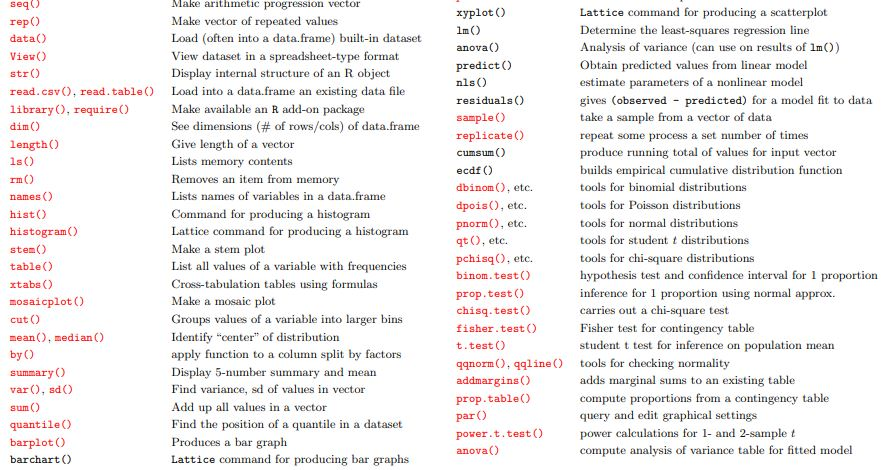
\includegraphics[width = 10.5cm]{use3.JPG} \\
\\
\vspace{0.5cm}

\footnotesize{\url{https://www.calvin.edu/~scofield/courses/m143/materials/RcmdsFromClass.pdf}}
\end{frame}



\section{Cheatsheets}
\begin{frame}{Cheatsheets}
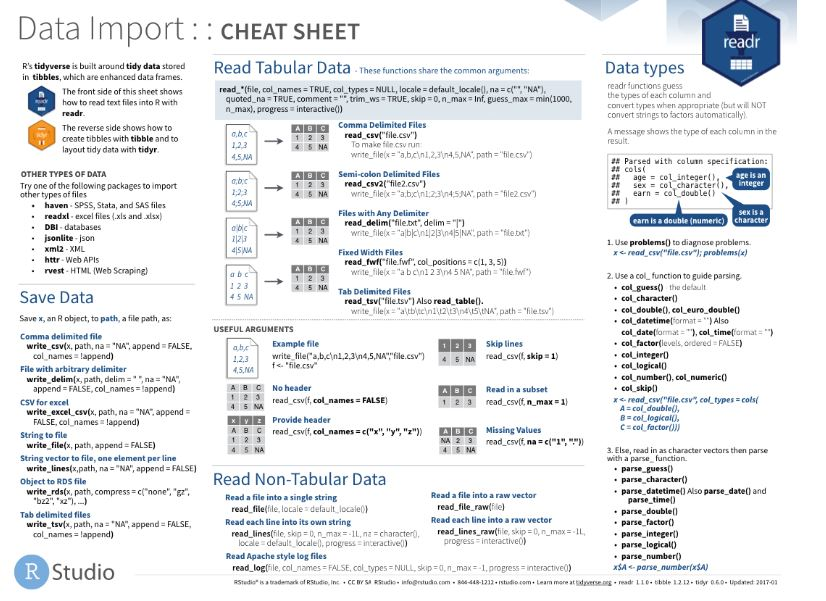
\includegraphics[width = 9cm]{ch.JPG} \\
\\
\url{https://www.rstudio.com/resources/cheatsheets/}
\end{frame}

\section{Help}
\begin{frame}{Help}
\begin{itemize}
    \item http://web.cs.ucla.edu/~gulzar/rstudio/basic-tutorial.html
    \item https://stats.idre.ucla.edu/r/modules/
    \item https://support.rstudio.com/hc/en-us/articles/200552336-Getting-Help-with-R \\
    \hspace{3cm} \\

\includegraphics[width = 5cm]{st.png} 
    \item https://stackoverflow.com/questions/tagged/rstudio
\end{itemize}
\end{frame}

\section{Further literature}
\begin{frame}{Further literature}

\hspace{3cm}
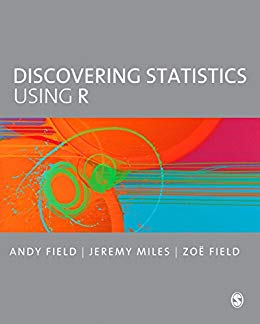
\includegraphics[width= 3cm]{ad.jpg}
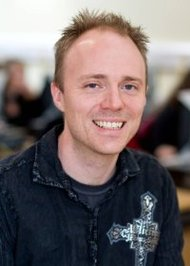
\includegraphics[width= 2.7cm]{af.jpg} \\
\vspace{1cm}
\\
Field, A. P., Miles, J., & Field, Z. (2012). \textit{Discovering statistics using R.}\\
\end{frame}

\section{Questions}
\begin{frame}{Questions?}
\vspace{-1.8cm}
    
\includegraphics[width = 10.5cm]{que.jpg} \\
\end{frame}


\ThankYouFrame

\end{document}